\documentclass[pmlr,twocolumn,10pt]{jmlr} % W&CP article

% ML4H 2026 track. Proceedings = 8pp excl. references/appendices, PMLR, archival.
% Unaccepted Proceedings submissions are automatically considered for Findings;
% the reverse is not true, so Proceedings is strictly the better submission.
\mlhtrack{proceedings}

\newif\iffinal
\finalfalse   % SUBMISSION: anonymous. \linenumbers is switched on below.
% \finaltrue  % camera-ready only

\iffinal
    \ifmlhneedspmlr
      \jmlrvolume{XXX}
      \jmlryear{2026}
    \fi
    \ifmlhfindings \jmlrproceedings{}{ML4H 2026 - Findings Track}\fi
    \ifmlhdemo     \jmlrproceedings{}{ML4H 2026 - Demo Track}\fi
    \jmlrworkshop{Machine Learning for Health (ML4H) 2026}
\else
    \jmlrproceedings{}{Submitted to ML4H 2026: \mlhtrackname}
    \jmlrworkshop{Machine Learning for Health (ML4H) 2026}
\fi

% amsmath, amssymb, natbib, graphicx, url, algorithm2e load automatically.
\urlstyle{same}
\usepackage{booktabs}
% siunitx is in the ML4H template for decimal-aligned table columns. It is not
% installed in every TeX distribution (Overleaf has it). Re-enable if the results
% tables need S columns.
%\usepackage{siunitx}
\usepackage[switch]{lineno}

\title[A Free Rescore Is Not Free]{A Free Rescore Is Not Free: A
  Benchmark-Recommended Score Substitution Reverses Sign Across Medical
  Imaging Datasets}

\author{Anonymous Author(s)}

\begin{document}

% Line numbers for review only. Loading `lineno` is not enough -- the template calls
% \linenumbers explicitly, and reviewers quote line numbers back to authors.
\iffinal\else\linenumbers\fi

\maketitle

\begin{abstract}
Unsupervised anomaly detection on medical images is reported as a contest between
named methods, but every reconstruction-based detector bundles two separable
decisions: the objective the model is trained to reconstruct, and the rule that turns
the residual into a score. The literature moves them together. The one exception ---
substituting a structural similarity residual into models trained under pixel
objectives --- is recommended in a current benchmark on the grounds that it improved
every model it was applied to. We test that claim. Reproducing ten methods under one
protocol and crossing four training objectives with five anomaly scores on three
datasets (RSNA, VinDr-CXR, LAG; $64\times64$, three seeds), we find the substitution
improves AUROC by 9.08 points on RSNA and harms it by 2.37 and 10.54 points on the
other two; all three are Holm-significant under paired DeLong tests and they disagree
in sign. The disagreement is not a modality effect: the two chest radiograph
collections differ from each other in sign. On the fundus data the substitution costs
two fifths of the cases the detector flags at a fixed false-positive rate, with
sensitivity at 95\% specificity falling from 21.9\% to 12.6\%. Two further
design-level comparisons reverse across datasets while four
replicate three of three. A variance head fitted to a frozen autoencoder shows what an
uncertainty score computes: residual relative to expected difficulty. A configuration
selected on RSNA and applied unchanged elsewhere gains 1.33 AUROC over the strongest
single method (95\% CI [0.41, 2.25]; six of six held-out seed measurements positive).
We do not reach the benchmark's best reported accuracy; we report what it is made of.
\end{abstract}

\begin{keywords}
anomaly detection, medical imaging, evaluation, reproducibility, autoencoders
\end{keywords}

\paragraph*{Data and Code Availability}
This study uses three public, de-identified benchmark datasets in the preprocessed form
released with the MedIAnomaly benchmark \citep{cai2025medianomaly}: the RSNA Pneumonia
Detection Challenge \citep{shih2019rsna}, VinDr-CXR \citep{nguyen2022vindr}, and LAG
\citep{li2019lag}. No new data were collected. Anonymized code, per-run manifests, and
the per-image anomaly score vectors for every reported cell are provided as supplemental
material; the score vectors are sufficient to recompute every table in this paper, and to
place a new anomaly score in the grid, without retraining any model.

\paragraph*{Institutional Review Board (IRB)}
This research does not require IRB approval. It is a secondary analysis of three public,
fully de-identified imaging benchmarks that were released for methodological research and
contain no identifiable private information; no human subjects were recruited, no
protected health information was accessed, and no clinical intervention or deployment was
involved.

\section{Introduction}
\label{sec:intro}

Unsupervised anomaly detection promises something a supervised classifier cannot offer in
medicine: a detector trained only on normal images, which does not require an annotated
example of every pathology it must eventually flag. The dominant recipe is
reconstruction. Train an autoencoder on healthy images, present it with a new image, and
treat whatever the model fails to reproduce as evidence of abnormality. A decade of work
has produced a long list of named methods built on that recipe, and benchmarks that rank
them \citep{baur2021autoencoders, lagogiannis2024unsupervised, cai2025medianomaly}.

The setting is not incidental. Unsupervised detection is proposed for precisely the
places where labels run out: triaging an imaging worklist that no reader can clear in
full, or screening for a condition whose positive examples nobody has yet annotated.
Health data supplies what the method needs, normal studies in quantity, and withholds
what supervision needs, an annotated instance of every pathology that must eventually be
flagged. More than half of prevalent glaucoma is undetected in every region studied
\citep{soh2021undetected}, and a team building a screen for it has few defensible design
choices and every reason to adopt a change a benchmark reports as free. On LAG, a fundus
collection whose labels come from glaucoma specialists reading intra-ocular pressure,
visual field and optic disc together, that change removes two fifths of the cases the
detector had been flagging at a fixed false-positive rate: sensitivity at 95\%
specificity falls from 21.9\% to 12.6\%. Neither figure is deployable, and we make no
deployment claim; the point is the size and the direction of what a scoring rule
silently decides. Sites differ in scanner, acquisition and case mix, and a rule
validated at one is applied at the next.

The ranking hides a design decision. A reconstruction-based detector uses a distance
function twice, in two different roles. It appears once as the training objective, where
it determines what the model is rewarded for reproducing, and again as the anomaly score,
where it determines how the residual is converted into a number. Nothing requires the two
to be the same function. In published work they almost always are, and they are changed
together. \citet{bergmann2019improving} state the design plainly --- their contribution is
obtained ``by adapting the loss \emph{and} evaluation functions'' --- and then attribute
the resulting improvement, from 0.688 to 0.966 AUC, to ``merely changing the loss
function''. Two things moved; one was credited. The practice has not gone away:
\citet{fan2025ssim} substitute SSIM for MSE in both roles at once in 2025.

If the two roles are never separated, no reported gain in this family can be assigned to
either. \citet{cai2025medianomaly} come closest, tabulating the training loss and the
anomaly score as separate columns, but every reconstruction method they evaluate
instantiates the two with the same distance. The off-diagonal --- train under one
distance, score under another --- has been entered once, and not as an experiment.
\citet{lagogiannis2024unsupervised} substitute an SSIM residual into four models trained
under pixel-space objectives, on the reasonable grounds that SSIM captures texture and
structure that absolute error does not, and report that this ``increased the performance
of all selected models it was applied to''. It is a sensible design decision, honestly
described. It is also a universal claim about a score substitution, tested on the datasets
that study used, and offered to readers as a default.

We test it. We reproduce ten methods from the MedIAnomaly benchmark under a single
protocol, then cross four training objectives with five anomaly scores on one backbone,
so that each decision can be varied while the other is held fixed. Rescoring costs no
training: the model is already fitted, and only the function applied to its residual
changes. We run the resulting grid on three datasets --- two chest radiograph collections
and one retinal fundus collection --- and compare cells with paired DeLong tests, with
Holm correction inside each dataset.

The substitution does not behave as reported. Rescoring a plain autoencoder with SSIM
improves AUROC by 9.08 points on RSNA, and harms it by 2.37 points on VinDr-CXR and 10.54
points on LAG. All three are Holm-significant, and they do not agree in sign. This is not
a power failure and not seed noise: the effects are an order of magnitude larger than the
seed-level spread, and the sign is consistent across all three seeds within each dataset.
Nor is it a difference between imaging modalities. RSNA and VinDr-CXR are both chest
radiograph collections, drawn through the same preprocessing pipeline, read by the same
backbone at the same resolution with the same seeds, and they disagree with each other in
sign. What separates the best from the worst outcome of one free substitution is 19.6
AUROC points. A free rescore is not free. Its direction is a property of the data, and must be validated
per dataset rather than inherited from a benchmark.

That result generalises into the paper's organising question: which conclusions about
these design decisions survive a change of dataset? Applying seven design-level
comparisons unchanged to all three datasets, four replicate in all three and three
reverse. We report both in one table. Among the reversals is a mechanism we proposed
ourselves --- that the residual advantage of jointly trained uncertainty estimation over a
post-hoc variance head reflects co-adaptation between reconstruction and variance during
training. That account predicts a gap on every dataset. On LAG there is none.

Alongside what fails to transfer, we establish what does. Fitting a variance head to a
completely frozen autoencoder recovers a large part of the advantage of a jointly trained
uncertainty model, on all three datasets, and lets us inspect what an uncertainty-weighted
score computes: not error magnitude, but residual relative to expected difficulty. And a
configuration chosen on RSNA --- head width and ensemble membership --- applied unchanged
to the two datasets it was not chosen on, gains 1.33 AUROC over the strongest single
method (95\% CI [0.41, 2.25]; six of six held-out seed measurements positive).

\paragraph*{Contributions.}
\begin{itemize}
\item A correction to a published recommendation: a benchmark-endorsed, no-retraining
  score substitution reverses sign across datasets, with all three directions significant
  under paired tests (\sectionref{sec:results}).
\item A design-decision replication table across three datasets in which four comparisons
  replicate and three reverse, reported with equal prominence.
\item The objective-by-score factorial as an attribution instrument, showing the two
  decisions are not additive: their interaction exceeds both main effects.
\item Evidence that mismatching objective and score is actively harmful rather than merely
  suboptimal --- a perceptually trained model read in pixel space scores below chance.
\item A frozen-backbone variance-head probe, and the reading of the uncertainty score it
  supports; a held-out transfer result; and a released instrument that places a new
  objective or score in the grid from stored score vectors, without a GPU.
\end{itemize}

\paragraph*{Scope.}
Every comparison here is internal to image-reconstruction detectors at $64\times64$
resolution with image-level labels, on one backbone whose architecture and
hyperparameters we inherit unchanged from the benchmark so that the reproduction remains
valid and the factorial stays free of confounds. The best accuracy reported on this
RSNA split belongs to a feature-reconstruction method that uses ImageNet weights, and we
do not reach it. That is the expected outcome for this study: a number and an explanation
are different products, and the design that produces the best number --- changing the
representation and the score in one step --- is precisely the design our results show
cannot be attributed. Three datasets, two of them chest radiographs, support no general
law of transfer. They are enough to exhibit one specific, quantified, twice-significant
failure of it.

\section{Related Work}
\label{sec:related}

We group prior work by which design decision it varied, because that is the axis along
which our contribution is defined.

\paragraph*{Varying the architecture, holding the residual fixed.}
The comparative studies that established this field vary what the model is, not how its
output is read. \citet{baur2021autoencoders} evaluate roughly a dozen autoencoder, VAE and
GAN variants on four brain MRI datasets under a unified pipeline, and find architectural
sophistication buys less than the literature implied. Their residual distance is $\ell_1$
throughout. They do vary the anomaly-extraction procedure --- reconstruction against
Monte-Carlo consensus, gradients and iterative restoration on fixed models --- but that
changes how the residual is \emph{obtained}, not the distance function that measures it.
\citet{lagogiannis2024unsupervised} extend this style of audit across modalities and
resolutions, and argue preprocessing and resolution dominate method identity.

\paragraph*{Varying the score, holding the objective fixed.}
That a trained model admits more than one readout is not new, and we do not claim it.
\citet{zimmerer2019unsupervised} keep a single variational autoencoder and derive several
anomaly scores from different terms of its evidence lower bound: the reconstruction error,
the KL term, and gradients of each with respect to the input. The objective never changes;
what changes is which term of it is differentiated. This is a genuine decoupling of score
from objective, and it establishes the score as a free variable. It is also a decoupling
along a different axis from ours: the choice is which part of one fixed objective to read,
not which distance function does the reading. \citet{meissen2022pitfalls} argue from the
other direction that the pixel residual is a poor anomaly score in the first place, because
it is dominated by reconstruction error on normal structure rather than by pathology. Their
critique motivates our question without answering it: they show the residual is
problematic, not which of its two roles is responsible.

\paragraph*{Varying the distance function --- on both axes at once.}
The reconstruction metric itself has been varied, but almost always in both roles
simultaneously. \citet{bergmann2019improving} are explicit about the design: their gain
comes ``by adapting the loss \emph{and} evaluation functions'' to capture local
inter-dependencies between image regions. The results sentence then reports that ``by
merely changing the loss function, the achieved AUC improves from 0.688 to 0.966''. Both
statements are in the same paper and both are accurate descriptions of what was done; only
the second is an attribution, and it credits one of two simultaneous changes. This is not a
historical artefact. \citet{fan2025ssim} substitute SSIM for mean squared error in both the
training objective and the anomaly score in a 2025 video anomaly detection study.
\citet{cai2025medianomaly} come closest to separating the two: their comparison tabulates
the training loss and the anomaly score as distinct columns, and they state that earlier
studies ``do not explicitly compare the effects of different distance functions''. But in
every reconstruction method they evaluate the two columns hold the same distance, so their
grid is populated only on its diagonal. They also report, at the level of the objective,
that a perceptual loss beats $\ell_2$ on several datasets and loses to it on another ---
dataset-dependence of the distance function, established for the training role.

\paragraph*{The one off-diagonal cell in the literature.}
\citet{lagogiannis2024unsupervised} enter the off-diagonal directly. For their
residual-based methods --- several of which optimise pixel-space objectives --- they
replace the pixel-wise absolute error with a structural similarity residual at scoring
time, on the grounds that SSIM accounts for texture and structure and not only luminance,
and they report that ``this change increased the performance of all selected models it was
applied to''. The substitution is reported in a subsection on residual extraction and
post-processing: a design decision, made once, described honestly, and offered as a
default. It is, to our knowledge, the only published instance of training under one
distance function and scoring under another in this literature, and it comes with a
universal claim attached. It is that claim we test, on three datasets, with paired tests.

\paragraph*{What remains open.}
Prior work varies the architecture with the residual fixed, the readout with the objective
fixed, or the distance in both roles together; one study varies the distance in the scoring
role alone. No study we could find, in medical, industrial or video anomaly detection,
evaluates the two as a crossed design. \citet{behrouzi2023anomaly} come close --- industrial
thermal autoencoders trained under both MSE and SSIM objectives, reported under three
anomaly scores --- but their results are indexed by score alone, so no loss-by-score
attribution can be recovered. Without the cross, a reported gain in this family cannot be
assigned to the objective, to the score, or to their interaction; and, as we show, cannot be
assumed to keep its sign on the next dataset.

\section{Method}
\label{sec:method}

\paragraph*{Two roles for one distance.}
A reconstruction-based detector is a map $f$ fitted on normal images and a scoring
functional applied to its output. Fitting minimises a distance
$d_{\mathrm{train}}(x, f(x))$ over normal data; scoring assigns
$s(x) = d_{\mathrm{score}}(x, f(x))$, larger meaning more anomalous. Published methods set
$d_{\mathrm{train}} = d_{\mathrm{score}}$ and report one number. We do not tie them.

\paragraph*{The grid.}
We cross four objectives --- $\ell_2$, SSIM, a VGG-19 relative perceptual distance, and a
heteroscedastic Gaussian likelihood --- with five scores: the same four, plus the
gradient-based score of \citet{zimmerer2019unsupervised}. \figureref{fig:factorial} gives the
design and names the published method each diagonal cell instantiates. Of $4\times5=20$
cells, 17 are defined. The three that are not are the uncertainty score applied to the
three objectives that produce no variance output; \sectionref{sec:probe} supplies them by
another route.

Off-diagonal cells involve no training. The weights fitted under $d_{\mathrm{train}}$ are
loaded frozen and only the scoring functional changes, so a row of the grid costs one
training run and four evaluations. This is what makes the factorial affordable, and it
means every off-diagonal cell is exactly reproducible from released weights.

\paragraph*{A variance head on a frozen backbone.}
\label{sec:probe}
The uncertainty score $s(x) = \mathrm{mean}[\exp(-\log\sigma^2)\,(x-\hat{x})^2]$ requires a
per-pixel variance that only a heteroscedastic model emits. To obtain that score for
backbones that do not, we attach a small convolutional head to an
\emph{already-trained, fully frozen} autoencoder and fit only the head, on normal training
images, under the heteroscedastic Gaussian negative log-likelihood
\citep{nix1994estimating,kendall2017uncertainties}. Every encoder and decoder weight is
frozen and the module is re-asserted into evaluation mode at each epoch, so batch
normalisation statistics cannot drift and the reconstruction is bit-identical to the parent
run. At $w{=}2$ the head is 14{,}528 parameters, 0.62\% of the backbone.

The probe carries three controls. A \emph{capacity} control sweeps
$w\in\{1,2,4,8,16\}$ (\sectionref{sec:selection}); $w{=}1$ reduces to a single transposed
convolution with normalisation and nonlinearity stripped, and fails everywhere, which makes
the threshold one of nonlinearity rather than capacity. A \emph{backbone-transfer} control
fits the same head to a perceptually trained backbone, where it fails by 30.6 AUROC ---
bounding the claim to pixel-space objectives. Finally, the head is compared both against the
parent it was fitted onto and against a jointly trained uncertainty model; these are
different claims and we label every result with its parent backbone throughout.

\section{Experimental Setup}
\label{sec:setup}

\paragraph*{Inherited protocol.}
Splits, backbone, preprocessing and every hyperparameter come unchanged from
\citet{cai2025medianomaly}: $64\times64$ inputs scaled to $[-1,1]$, a 16-dimensional latent,
250 epochs, Adam at $10^{-3}$, batch size 64, three seeds (42, 43, 44). We inherit rather
than tune because it is what makes the reproduction valid and the factorial free of
confounds: within the grid, only the objective and the score differ.

\paragraph*{Datasets.}
RSNA \citep{shih2019rsna} and VinDr-CXR \citep{nguyen2022vindr} are chest radiograph
collections; LAG \citep{li2019lag} is retinal fundus photography with glaucoma labels
assigned by specialists from intra-ocular pressure, visual field and optic disc assessment.
Training uses normal images only. Test sets are balanced by construction: 1000/1000 for
RSNA and VinDr-CXR, 811/811 for LAG. That prevalence is a benchmark artifact, not a clinical
one, and we return to it in \sectionref{sec:results}.

\paragraph*{Reproduction as calibration.}
Before crossing anything we reproduced ten published methods under this protocol. Nine of
ten fall within one standard deviation of their published values on RSNA, four within 0.2
AUROC, with matching parameter counts; the exception is a denoising autoencoder run at a
single seed, which cannot separate an implementation gap from seed variation, and which we
report rather than drop. The full table is in the appendix. The reproduction is not a
contribution. It is the calibration that licenses the rest: cells of the grid are comparable
to published numbers only if the diagonal reproduces them.

\paragraph*{Held-out configuration.}
Two choices in this paper are ours rather than inherited: the head width and the ensemble
membership. Both were fixed on RSNA, written to a machine-readable selection card, and
applied unchanged to VinDr-CXR and LAG, which were run afterwards. No entry was revised.
Nothing else is chosen --- everything not on that card is inherited --- which bounds the
selection surface to two integers. The card and the per-seed held-out records produced at
run time are released with the code.

\paragraph*{Statistics.}
We report the unit of analysis for every test, because the tests answer different questions.
Paired DeLong tests \citep{delong1988comparing}, computed with the fast algorithm of
\citet{sun2014fast}, treat the test \emph{images} as the sampling unit; they license
statements about two scoring rules on these images given these trained weights, and carry no
seed-variance component, so they say nothing about retraining. Seed-level paired $t$-tests
treat the \emph{seed} as the unit and do speak to retraining, but with three seeds they are
underpowered below roughly 1.5 AUROC: a null result there means unresolved, not equivalent.
Holm correction \citep{holm1979simple} is applied within each dataset, each dataset being a
separate replication. Sensitivity at fixed specificity uses a split-half protocol --- the
threshold is estimated on one half of the test set and sensitivity measured on the other,
over 500 stratified splits --- with paired image-level bootstrap intervals in which the
threshold is recomputed inside every replicate. We do not compute $t$-intervals over three
seeds; per-seed values are reported instead.

\subsection{Selection discipline}
\label{sec:selection}

One quantity in this paper was fixed by looking at test performance. The variance head has a
width parameter, and we set it to $w{=}2$ after inspecting RSNA test AUROC across
$w\in\{1,2,4,8,16\}$. A paper arguing that design decisions are validated on the wrong data
should state its own instance first, and then state what follows.

Three things follow. First, the quantity inspected is flat. The RSNA sweep reads 66.9, 82.0,
82.1, 81.8, 78.2; width 1 is below the useful range and width 16 carries one diverged seed,
but $w\in\{2,4,8\}$ spans 0.24 AUROC. The inspection could not have discriminated inside
that plateau, and $w{=}2$ is not the sweep's maximum even on the dataset it was chosen on.
It is the smallest width at which the head works at all.

Second, the inspection did not flatter the held-out results. On VinDr-CXR and LAG, $w{=}4$
exceeds the inherited $w{=}2$ by 1.77 and 0.29 AUROC. Whatever the RSNA inspection bought,
it cost on both datasets we report as held out.

Third, a rule that never reads a test image chooses differently and does no worse. Selecting
the width by the head's final training negative log-likelihood, computed on normal training
images alone, ranks both failure widths last on all three datasets and selects $w{=}8$ on
RSNA; $w{=}8$ carried unchanged to the held-out pair averages 0.57 AUROC above $w{=}2$. The
criterion is a training-set quantity rather than a held-out one, since no validation split
was retained, but with the backbone frozen it fits fewer than 15{,}000 parameters, and it
ranks the widest head below the middle of the sweep on every dataset.

The width does not enter the transfer result: that ensemble's members are the perceptual and
uncertainty models, neither of which carries a head.

\section{Results}
\label{sec:results}

\subsection{The substitution reverses, and what that costs}

Rescoring a trained autoencoder with SSIM changes nothing about the model. The weights are
the parent run's, the reconstruction is bit-identical, and only the function applied to the
residual differs. On RSNA that change is worth $+9.08$ AUROC. On VinDr-CXR it is worth
$-2.37$, and on LAG $-10.54$. All three are Holm-significant under paired DeLong
(\tableref{tab:replication}), and 19.6 AUROC points separate the best outcome from the worst.

The disagreement is not between imaging modalities. RSNA and VinDr-CXR are both chest
radiograph collections, drawn through one preprocessing pipeline, read by one backbone at one
resolution with the same three seeds, and they disagree in sign with each other. Nor is it
seed noise: within each dataset all three seeds agree in sign, and the effects are an order
of magnitude larger than the seed-level spread.

It is also not an artefact of the summary metric. Estimating a threshold at 95\% specificity
on one half of the test set and measuring sensitivity on the other, over 500 stratified
splits, the substitution moves sensitivity from 17.7\% to 31.2\% on RSNA, from 13.6\% to
10.9\% on VinDr-CXR, and from 21.9\% to 12.6\% on LAG --- on the fundus data, two fifths of
the cases the detector had been flagging. Neither LAG figure is deployable: published
glaucoma screening operates near 85\% sensitivity at this specificity, and we make no
deployment claim. What the operating point establishes is that a change described as free
is not neutral at the point where a detector would actually be used.

One dataset separates the two readings. On VinDr-CXR the AUROC difference is
Holm-significant while the operating-point difference is not, with two of three per-seed
bootstrap intervals crossing zero. We report that rather than resolve it: a summary metric
and a deployment-relevant operating point can disagree, which is itself a reason not to read
AUROC alone.

\subsection{What replicates and what reverses}

Applying seven design-level comparisons unchanged to all three datasets, four replicate in
sign with Holm significance everywhere and three reverse (\tableref{tab:replication}). We
call a comparison replicated when it agrees in sign \emph{and} clears Holm correction on all
three datasets; magnitudes are not required to agree, and they do not. The head improves on
frozen AE-SSIM by $+1.19$ on RSNA and $+15.92$ on LAG --- a thirteen-fold spread under one
verdict. Sign is considerably more portable than magnitude.

Grouping the rows by the decision under test shows the instability is not spread evenly.
The four comparisons that replicate all measure a construction against something it is
built on top of: a head against the frozen backbone it was fitted onto, an ensemble against
a member it contains. The three that reverse all compare arms where neither contains the
other --- a score substituted for another on identical weights, or a post-hoc construction
against a jointly trained one. We return to this in \sectionref{sec:discussion}.

\begin{table}[t]
\centering\footnotesize
\caption{Design-level comparisons applied unchanged to three datasets. Values are AUROC
point differences; positive favours the first-named method. Paired DeLong tests on the test
images, Holm-corrected within each dataset; \textsuperscript{*} significant at $0.05$;
\textsuperscript{\dag} $p_{\mathrm{Holm}}=0.055$, underpowered at three seeds --- direction
unresolved, not absent. DeLong conditions on these trained models and carries no
seed-variance component; per-seed values are in the appendix. Four comparisons replicate in
sign across all three datasets and three reverse.}
\label{tab:replication}
\begin{tabular}{@{}l@{\hspace{4pt}}r@{\hspace{5pt}}r@{\hspace{5pt}}r@{}}
\toprule
Comparison & RSNA & VinDr & LAG \\
\midrule
\multicolumn{4}{@{}l}{\emph{Score substitution}}\\
\quad AE rescored w/ SSIM vs.\ AE & $+9.08^{*}$ & $-2.37^{*}$ & $-10.54^{*}$ \\[2pt]
\multicolumn{4}{@{}l}{\emph{Head vs.\ the backbone it is fitted onto}}\\
\quad head vs.\ frozen AE & $+13.65^{*}$ & $+12.38^{*}$ & $+4.31^{*}$ \\
\quad head vs.\ frozen AE-SSIM & $+1.19^{*}$ & $+13.95^{*}$ & $+15.92^{*}$ \\[2pt]
\multicolumn{4}{@{}l}{\emph{Head vs.\ joint training}}\\
\quad AE-U vs.\ head on AE & $+4.86^{*}$ & $+5.72^{*}$ & $-0.78^{\dag}$ \\
\quad head on AE-SSIM vs.\ AE-U & $+0.13$ & $-1.03$ & $-4.35^{*}$ \\[2pt]
\multicolumn{4}{@{}l}{\emph{Score ensembling}}\\
\quad ensemble vs.\ AE-PL & $+1.16^{*}$ & $+1.57^{*}$ & $+1.08^{*}$ \\
\quad ensemble vs.\ AE-U & $+1.88^{*}$ & $+2.95^{*}$ & $+4.49^{*}$ \\
\bottomrule
\end{tabular}
\end{table}

\subsection{Attribution: what the objective buys}

\figureref{fig:factorial} gives the full grid on RSNA. The four boxed cells are the diagonal,
where every published method in this family sits, because every one sets
$d_{\mathrm{train}}=d_{\mathrm{score}}$. Everything else is off-diagonal.

The two decisions are not additive. Taking the plain autoencoder as reference, changing only
the score to SSIM is worth $+9.08$; changing only the objective to SSIM, while still scoring
with $\ell_2$, is worth $-6.45$; doing both --- which is AE-SSIM --- is worth $+12.46$. The
joint effect exceeds the sum of the single changes by 9.8 AUROC points. We report this as a
descriptive additivity check in AUROC points relative to a fixed reference, not as an
analysis of variance: it carries no error model, and AUROC is bounded and not additive. The
same arithmetic for the perceptual pair gives 35.2 points, but that figure is inflated by a
constituent cell sitting below chance, where AUROC's geometry differs, and we do not lean on
it.

An objective does not produce a better reconstruction that any score can read. It constrains
some directions and leaves others free, and a score is informative only in the directions
that were constrained. The perceptual row is the clearest case: read with $\ell_2$ it gives
44.9 and read with SSIM 44.0, both below chance, and both replicate --- the same cells give
38.7 and 34.7 on VinDr-CXR. Below chance is not the absence of signal but its inversion:
44.9 carries as much information as 55.1 would, with the sign reversed. That is the practical
point. A scoring rule inherited without validation may not merely underperform; it may rank
the wrong images first, and nothing in the score itself reveals which.

\begin{figure}[t]
\centering
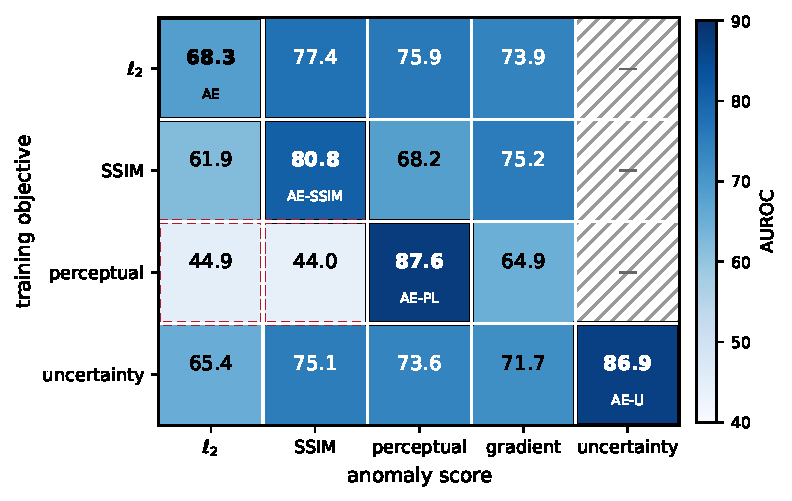
\includegraphics[width=\linewidth]{figures/factorial_rsna.pdf}
\caption{The objective $\times$ score grid on RSNA, AUROC averaged over three seeds. Boxed
cells are the diagonal and name the published method they instantiate. Red dashed cells are
below chance. Hatched cells are undefined: the uncertainty score requires a per-pixel
variance that only the heteroscedastic objective emits, and \sectionref{sec:probe} supplies
them by fitting a variance head to a frozen backbone. The grid was run on all three datasets
at three seeds; RSNA is shown here and the other two are in the appendix.}
\label{fig:factorial}
\end{figure}

\subsection{What the uncertainty score computes}

The variance head lets us ask what an uncertainty-weighted score is measuring. It is not
error magnitude. Across the test set the predicted log-variance correlates with the image's
own mean residual at $\rho=0.51$, so harder images are discounted --- yet abnormal images
receive a \emph{smaller} log-variance than normal ones ($-0.0997$), and are therefore
discounted less than their residual alone would predict. The score is a residual relative to
the difficulty the model expected, and the anomaly signal is the gap between the two.

Four controls separate this from simpler explanations, on RSNA. The full head reaches 82.00.
Reduced to a single scalar per image, discarding all spatial structure, it reaches 79.87 ---
so most of the benefit is a per-image calibration rather than a spatial uncertainty map. A
static map fixed to the training-set mean residual gives 69.10, and zero-parameter whitening
by the mean residual gives 69.59, against the plain autoencoder's 68.35. The head is
therefore neither an anatomical prior nor a trivial normalisation.

\subsection{Held-out transfer, and its failed extension}

Two choices were fixed on RSNA and applied unchanged elsewhere. A rank-average of the
perceptual and uncertainty scores gains 1.33 AUROC over the strongest single method on the
two datasets it was not fixed on (six of six seed measurements positive, seed-level 95\% CI
$[0.41, 2.25]$) --- though with dataset as the unit of analysis $n=2$, which supports the
observation that both held-out datasets agree in sign and supports no $p$-value.

The same protocol refuses an extension. Adding a third member gains $+0.72$ on RSNA, where
the combination was selected, and loses $1.26$ on held-out LAG. We report the extension
because the contrast is the paper's own argument applied to its own results: a gain measured
where a choice was made is not evidence that the choice transfers, and the only way to tell
the two apart is to fix the configuration first and look afterwards.

\section{Discussion}
\label{sec:discussion}

\paragraph*{One distance function, two roles, one answer.}
SSIM enters this study twice, and both entries move together. Measured against the plain
autoencoder on each dataset, using SSIM as the score is worth $+9.08$, $-2.37$ and $-10.54$;
using it as the objective is worth $+12.46$, $-1.56$ and $-11.61$. The signs agree on all
three datasets and the magnitudes are within 3.4 points. Once the residual is read with
SSIM, which objective produced it changes the answer by at most 3.4 AUROC and on two
datasets by about one. What moves is the level of the whole SSIM column, and it moves by
dataset. The reversal is therefore a property of what SSIM can read in these residuals
rather than of the role SSIM is given, which is the paper's thesis in its sharpest form: two
independent routes into the same column land within about a point of each other. We do not
explain why SSIM reads chest radiograph residuals well and fundus residuals poorly. Spatial
scale of the structures involved and the ratio of the SSIM window to the image are the
obvious candidates, and we have not separated them.

\paragraph*{Where the instability lives.}
The partition in \tableref{tab:replication} aligns exactly with whether one arm is built on
top of the other: four additive comparisons replicate, three substitutive or cross-family
comparisons reverse. We noticed this after the fact, on seven comparisons chosen for other
reasons, so it is a hypothesis rather than a result. We state it because it is checkable. It
predicts that a further additive comparison should hold its sign on a fourth dataset, and
that a further substitution should not.

\paragraph*{What follows for practice.}
A scoring rule is not a property of a method that travels with it. Before adopting a rescore
reported as free, measure it on labelled data from the site where it will run; and where no
labelled data exists, do not adopt it, because the two chest radiograph collections here
disagree with each other and there is no cheaper way to learn which case you are in. The
converse is worth as much: additive constructions held their sign on every dataset we tried,
and that is the one class of change this evidence supports carrying across sites unvalidated.

\paragraph*{What we do not explain.}
Why the SSIM column's level depends on the dataset; whether any of this survives a change of
resolution, which we address below; whether the additive/substitutive partition is real or
an artefact of seven comparisons; and anything about localisation or deployment. The
operating-point analysis says what a scoring choice costs at a fixed false-positive rate. It
does not say that either configuration should be used.

\section{Limitations}
\label{sec:limitations}

\textbf{1. Resolution, and a windowed score.} All comparisons are at $64\times64$, inherited
from the benchmark, which reports that this resolution ``achieves comparable performance to
using a larger input size, such as $128\times128$'' \citep{cai2025medianomaly}. That ablation
varies resolution under pixel-space objectives and pixel-space scores. SSIM is computed over
an $11\times11$ window, which at $64\times64$ spans roughly a sixth of the image, and no
published ablation covers whether a windowed score behaves the same way at both resolutions.
This is the sharpest alternative reading of our central result, so we tested it directly at
fixed resolution by recomputing the SSIM score on identical weights and reconstructions with
smaller windows. Shrinking the window does not attenuate the reversal; it amplifies it.
Against the $\ell_2$ baseline, the rescore is worth $+9.03$, $+7.87$ and $+3.86$ on RSNA at
windows of 11, 7 and 5, and $-10.66$, $-11.12$ and $-14.41$ on LAG. The sign disagreement
between RSNA and the other two datasets survives at all three, and only disappears at a
$3\times3$ window, where SSIM is worse than plain $\ell_2$ everywhere. An $11\times11$ window
at $128\times128$ would span 8.6\% of the image, between our $5\times5$ and $7\times7$
settings, where the disagreement is still present; we therefore expect the reversal to
persist at higher resolution with a smaller positive side. That remains a prediction ---
raising the resolution also changes the image content, not only the window ratio --- and the
replication is the first item of further work.

\textbf{2. Three datasets.} We claim no general law of transfer. We exhibit one specific,
quantified failure of it, significant in both directions. The panel's two most similar
members disagree with each other, so the result is not reducible to imaging modality, but
three datasets cannot establish how often such reversals occur.

\textbf{3. Three seeds, and the unit of analysis.} DeLong tests condition on these trained
models and carry no seed-variance component; claims below roughly two AUROC points rest on
the seed-level column, where three seeds are underpowered. A non-significant seed-level
result is unresolved, not null: the LAG comparison of AE-U against the post-hoc head
($-0.78$, $p_{\mathrm{Holm}}=0.055$) is reported as direction unresolved.

\textbf{4. One backbone, untuned.} Architecture and hyperparameters are inherited and never
tuned. This is what makes the reproduction valid and the factorial free of confounds, but the
decomposition's stability under a different backbone is untested.

\textbf{5. Image-level labels only.} No localisation claim is made or supported, which suits
the triage and screening settings named in \sectionref{sec:intro} and no others.

\textbf{6. Balanced test sets.} 50\% prevalence is a benchmark construction. AUROC is
prevalence-invariant, so the headline is unaffected, but the operating points are read on a
balanced set and their sensitivities are not transportable to a screening cohort. LAG in
particular is a tertiary referral collection, whose case mix is more severe than a screening
population's.

\textbf{7. Selection.} One quantity was fixed by inspecting test performance; see
\sectionref{sec:selection}.

\textbf{8. One incomplete cell.} A single post-hoc head run on LAG failed a non-finite-loss
guard, so that comparison uses two seeds rather than three; it is marked wherever it appears.

\section{Conclusion}

Two decisions inside a reconstruction-based detector have been moving together, and the
literature has been crediting one of them. Separating them shows that the anomaly score
carries much of the reported gain and that its direction is not a property of the method: a
substitution a current benchmark recommends as free gains 9.08 AUROC points on one dataset
and loses 10.54 on another, and the two chest radiograph collections in our panel disagree
with each other. We do not offer a better detector. We offer the instrument that says which
part of one to believe, and we release the per-image score vectors so a reader can place a
new objective or a new score in the grid without a GPU.

\paragraph*{Use of AI Assistance}
We used a large language model as a coding and writing assistant: to help implement and
review the experiment harness, to draft and revise prose, and to cross-check claims
against our experimental record. It was not part of the method under study, and no
experimental result was produced by it. All experiments were executed by the authors on
the datasets described above. The authors verified every reported number against the
stored per-run outputs, and read and confirmed every cited work; the authors take full
responsibility for the content of this paper.

\appendix

\section{Per-seed differences}
\label{apd:perseed}
Every comparison in \tableref{tab:replication} as three individual seed measurements,
AUROC points, paired DeLong on identical images. The main text reports means; these are
the values behind them. Note the exceptions the means conceal: one RSNA seed for the head
against frozen AE-SSIM is negative, and the two comparisons of a post-hoc construction
against a jointly trained model disagree in sign \emph{within} a dataset --- which is why
the LAG row of the former is reported as direction unresolved rather than as no
difference. Across the four comparisons that replicate, 35 of 36 seed measurements agree
in sign.

\begin{table}[h]
\centering\footnotesize
\caption{Per-seed AUROC differences (seeds 42, 43, 44). A dash marks the single post-hoc
head run on LAG that failed a non-finite-loss guard and was not recorded.}
\begin{tabular}{@{}l@{\hspace{5pt}}r@{\hspace{6pt}}r@{\hspace{6pt}}r@{}}
\toprule
 & seed 42 & seed 43 & seed 44 \\
\midrule
\multicolumn{4}{@{}l}{\emph{AE rescored with SSIM vs.\ AE}}\\
\quad RSNA & $+8.80$ & $+8.96$ & $+9.47$ \\
\quad VinCXR & $-1.86$ & $-2.77$ & $-2.50$ \\
\quad LAG & $-9.55$ & $-10.93$ & $-11.13$ \\
\multicolumn{4}{@{}l}{\emph{head vs.\ frozen plain AE}}\\
\quad RSNA & $+13.87$ & $+13.75$ & $+13.33$ \\
\quad VinCXR & $+13.31$ & $+12.50$ & $+11.34$ \\
\quad LAG & $+1.94$ & $+5.47$ & $+5.52$ \\
\multicolumn{4}{@{}l}{\emph{head vs.\ frozen AE-SSIM}}\\
\quad RSNA & $+1.29$ & $+2.58$ & $-0.30$ \\
\quad VinCXR & $+14.88$ & $+14.84$ & $+12.12$ \\
\quad LAG & $+13.49$ & $+16.93$ & $+17.35$ \\
\multicolumn{4}{@{}l}{\emph{AE-U vs.\ head on frozen AE}}\\
\quad RSNA & $+4.16$ & $+3.98$ & $+6.46$ \\
\quad VinCXR & $+5.45$ & $+6.98$ & $+4.74$ \\
\quad LAG & $+0.48$ & $-2.50$ & $-0.32$ \\
\multicolumn{4}{@{}l}{\emph{head on AE-SSIM vs.\ AE-U}}\\
\quad RSNA & $+1.47$ & $-0.16$ & $-0.92$ \\
\quad VinCXR & $-1.32$ & $-3.24$ & $+1.48$ \\
\quad LAG & $-0.13$ & --- & $-8.57$ \\
\multicolumn{4}{@{}l}{\emph{ensemble vs.\ AE-PL}}\\
\quad RSNA & $+0.90$ & $+1.10$ & $+1.49$ \\
\quad VinCXR & $+1.96$ & $+2.52$ & $+0.25$ \\
\quad LAG & $+0.71$ & $+0.77$ & $+1.76$ \\
\multicolumn{4}{@{}l}{\emph{ensemble vs.\ AE-U}}\\
\quad RSNA & $+2.34$ & $+1.97$ & $+1.32$ \\
\quad VinCXR & $+2.32$ & $+1.90$ & $+4.61$ \\
\quad LAG & $+6.08$ & $+5.21$ & $+2.17$ \\
\bottomrule
\end{tabular}
\end{table}

\section{The factorial on the held-out datasets}
\label{apd:grids}
\figureref{fig:factorial} shows RSNA. The same 17 cells were run at three seeds on both
held-out datasets; they are given here. Rows are training objectives, columns anomaly
scores, bold marks the diagonal, and a dash marks the uncertainty score where no variance
output exists.

\begin{table}[h]
\centering\footnotesize
\caption{VinDr-CXR (upper) and LAG (lower), AUROC averaged over three seeds.}
\begin{tabular}{@{}l@{\hspace{4pt}}r@{\hspace{4pt}}r@{\hspace{4pt}}r@{\hspace{4pt}}r@{\hspace{4pt}}r@{}}
\toprule
objective & $\ell_2$ & SSIM & perc. & grad. & unc. \\
\midrule
\multicolumn{6}{@{}l}{\emph{VinDr-CXR}}\\
$\ell_2$ & \textbf{56.03} & 53.65 & 57.80 & 60.93 & --- \\
SSIM & 52.51 & \textbf{54.46} & 54.03 & 58.33 & --- \\
perceptual & 38.67 & 34.69 & \textbf{75.50} & 45.81 & --- \\
uncertainty & 55.71 & 51.12 & 53.96 & 61.26 & \textbf{74.13} \\
\midrule
\multicolumn{6}{@{}l}{\emph{LAG}}\\
$\ell_2$ & \textbf{78.96} & 68.43 & 66.74 & 78.67 & --- \\
SSIM & 46.28 & \textbf{67.35} & 49.77 & 43.13 & --- \\
perceptual & 53.90 & 43.38 & \textbf{85.90} & 54.28 & --- \\
uncertainty & 77.71 & 66.65 & 68.75 & 82.91 & \textbf{82.50} \\
\bottomrule
\end{tabular}
\end{table}

\section{Reproduction of the inherited baselines}
\label{apd:repro}
Ten published methods under the protocol of \citet{cai2025medianomaly}, RSNA, image-level
AUROC. The reference column is their Table~6 and is used only as a target to check our
implementations against. Nine of ten fall within one standard deviation; four within 0.2
points. The exception is the denoising autoencoder, which we ran at a single seed: one
seed cannot separate an implementation gap from seed variation, and we report it rather
than drop it.

\begin{table}[h]
\centering\footnotesize
\caption{Reproduction. Ours is mean $\pm$ population standard deviation over seeds; on
three seeds this understates the sample standard deviation by a factor of 1.22.}
\begin{tabular}{@{}lcrrr@{}}
\toprule
Method & $n$ & ours & reference & $\Delta$ \\
\midrule
AE             & 3 & $68.35\pm0.65$ & $67.5\pm0.9$ & $+0.85$ \\
AE-$\ell_1$    & 3 & $68.53\pm0.86$ & $68.1\pm0.4$ & $+0.43$ \\
AE-SSIM        & 3 & $80.81\pm0.35$ & $80.9\pm0.3$ & $-0.09$ \\
AE-PL          & 3 & $87.58\pm0.27$ & $87.5\pm0.2$ & $+0.08$ \\
VAE            & 3 & $67.33\pm1.41$ & $67.9\pm0.8$ & $-0.57$ \\
AE-U           & 3 & $86.86\pm0.44$ & $86.5\pm0.9$ & $+0.36$ \\
DAE            & 1 & $83.87$        & $86.1\pm0.7$ & $-2.23$ \\
AE-Grad        & 3 & $73.86\pm0.87$ & $73.7\pm1.0$ & $+0.16$ \\
VAE-Grad$_{\mathrm{rec}}$   & 3 & $71.68\pm1.11$ & $71.6\pm0.8$ & $+0.08$ \\
VAE-Grad$_{\mathrm{combi}}$ & 3 & $67.84\pm1.35$ & $67.4\pm0.3$ & $+0.44$ \\
\bottomrule
\end{tabular}
\end{table}

\section{Head width and the SSIM window}
\label{apd:sweeps}

\paragraph*{Width sweep.} The post-hoc variance head across five widths, three seeds, all
three datasets. Widths 2, 4 and 8 span 0.23, 1.77 and 0.78 AUROC on RSNA, VinDr-CXR and
LAG respectively. Width 1 reduces to a single transposed convolution with normalisation
and nonlinearity stripped and fails everywhere; width 16 is an optimisation failure, with
initial training losses across seeds spanning three orders of magnitude.

\begin{table}[h]
\centering\footnotesize
\caption{Post-hoc head AUROC by width. The width used throughout the paper is $w{=}2$;
see \sectionref{sec:selection}.}
\begin{tabular}{@{}lrrrrr@{}}
\toprule
 & $w{=}1$ & $w{=}2$ & $w{=}4$ & $w{=}8$ & $w{=}16$ \\
\midrule
RSNA      & 66.94 & 82.00 & 82.05 & 81.81 & 78.22 \\
VinDr-CXR & 52.49 & 68.41 & 70.18 & 70.03 & 64.50 \\
LAG       & 74.04 & 83.27 & 83.56 & 82.78 & 81.23 \\
\bottomrule
\end{tabular}
\end{table}

\paragraph*{SSIM window sweep.} The rescore recomputed on identical frozen weights and
reconstructions at four window sizes, at fixed $64\times64$. Values are AUROC differences
against the $\ell_2$ baseline on the same weights.

\begin{table}[h]
\centering\footnotesize
\caption{Effect of the SSIM rescore by window size. The sign disagreement between RSNA and
the other two datasets survives at windows 11, 7 and 5, and disappears at 3, where SSIM is
worse than $\ell_2$ everywhere.}
\begin{tabular}{@{}lrrr@{}}
\toprule
window (\% of image) & RSNA & VinDr-CXR & LAG \\
\midrule
$11\times11$ (17.2\%) & $+9.03$ & $-2.59$ & $-10.66$ \\
$7\times7$   (10.9\%) & $+7.87$ & $-3.52$ & $-11.12$ \\
$5\times5$   (7.8\%)  & $+3.86$ & $-5.78$ & $-14.41$ \\
$3\times3$   (4.7\%)  & $-5.49$ & $-10.82$ & $-22.36$ \\
\bottomrule
\end{tabular}
\end{table}

\section{Operating-point protocol}
\label{apd:oppoint}
Sensitivity at fixed specificity is reported under a split-half protocol: the test set is
split in half, stratified by label; the threshold achieving 95\% specificity is estimated
on the first half; sensitivity for both scoring rules is measured on the second; this is
repeated over 500 stratified splits and averaged, per seed. The threshold is therefore
never estimated on the data it is evaluated on. Confidence intervals come from a paired
image-level bootstrap in which the threshold is recomputed inside every replicate, since
fixing it at its point estimate would omit threshold-estimation uncertainty --- the
dominant term when estimating a far-tail quantile. We do not construct intervals over
three seeds; per-seed values are reported instead.

Balanced test sets mean these sensitivities are not transportable to a screening cohort.
LAG in particular is drawn from a tertiary referral population whose case mix is more
severe than a screening population's, and its labels come from specialists reading
intra-ocular pressure, visual field and optic disc together.

\bibliography{ref}

\end{document}
